\documentclass[a4paper, 12pt]{article}
\usepackage{titling}
\usepackage{array}
\usepackage{booktabs}
\usepackage{enumitem}
\usepackage{graphicx}
\usepackage{hyperref}
\usepackage{amssymb}
\usepackage{listings}
\usepackage{color} %red, green, blue, yellow, cyan, magenta, black, white
\setlength{\heavyrulewidth}{1.5pt}
\setlength{\abovetopsep}{4pt}
\setlength{\parindent}{0pt}
\graphicspath{{.}}

\usepackage[margin=1in]{geometry}
\definecolor{mygreen}{RGB}{28,172,0} % color values Red, Green, Blue
\definecolor{mylilas}{RGB}{170,55,241}
% Must be after geometry
\usepackage{fancyhdr}
\pagestyle{fancy}
\fancyhf{}
\rhead{SEE Assignment 4}
\lhead{P.Lukin, E. Ovchinnikova}
\cfoot{\thepage}

\setlength{\droptitle}{-5em}

\title{Scientific Experimentation and Evaluation  \\
				Assignment: 4}
\author{Petr Lukin, Evgeniya Ovchinnikova}
\date{Lecture date: $24^{th}$ October 2016}

\begin{document}
%-------------------------------------------------------------------------------
\lstset{language=Matlab,%
    %basicstyle=\color{red},
    breaklines=true,%
    morekeywords={matlab2tikz},
    keywordstyle=\color{blue},%
    morekeywords=[2]{1}, keywordstyle=[2]{\color{black}},
    identifierstyle=\color{black},%
    stringstyle=\color{mylilas},
    commentstyle=\color{mygreen},%
    showstringspaces=false,%without this there will be a symbol in the places where there is a space
    numbers=left,%
    numberstyle={\tiny \color{black}},% size of the numbers
    numbersep=9pt, % this defines how far the numbers are from the text
    emph=[1]{break},emphstyle=[1]\color{red}, %some words to emphasise
    %emph=[2]{word1,word2}, emphstyle=[2]{style},
}

%-------------------------------------------------------------------------------


\maketitle

\section{Experiment setup}

The current experiment was conducted using AICISS optical tracking system - three USB-cameras (lifecam19,20,22) mounted on the ceiling in a room C022. The cameras are pre-calibrated, so we didn't need to perform a calibration by ourselves as we did in the previous assignment. For this system usage we needed to install a marker that would be tracked by the system on the robot. We have generated some new markers (Fig. \ref{fig:markers}) and added them and their linear size (10 $\times$ 10 cm) to the dictionary: 

\begin{lstlisting}

dictionary.yml:

%YAML:1.0
nmarkers: 5
markersize: 4
marker_0: "0111000111100101"
marker_1: "1100011000010101"
marker_2: "0110101010001001"
marker_3: "0011001000011111"
marker_4: "0101010000111100"

see_robot.json

{
    "Markers":
    {
        "15402":
        [
            "70.0 -70.0",
            "70.0 70.0",
            "-70.0 70.0",
            "-70.0 -70.0"
        ]
    },
    "Dimensions":
    {
        "Length": "100",
        "Width": "100"
    }
}

\end{lstlisting}

\begin{figure}[h]
  \centering
  \caption{Two of newly generated markers.\label{fig:markers}}
  
\includegraphics[width=0.5\textwidth]{markers}
\end{figure}

It is important for the measurement that the marker is well fixed, doesn't shake and is parallel to the floor, so we've made the construction depicted in Fig. \ref{fig:markerHolder} to fix the marker on it.

\begin{figure}[h]
  \centering
  \caption{A marker holding construction.\label{fig:markerHolder}}
  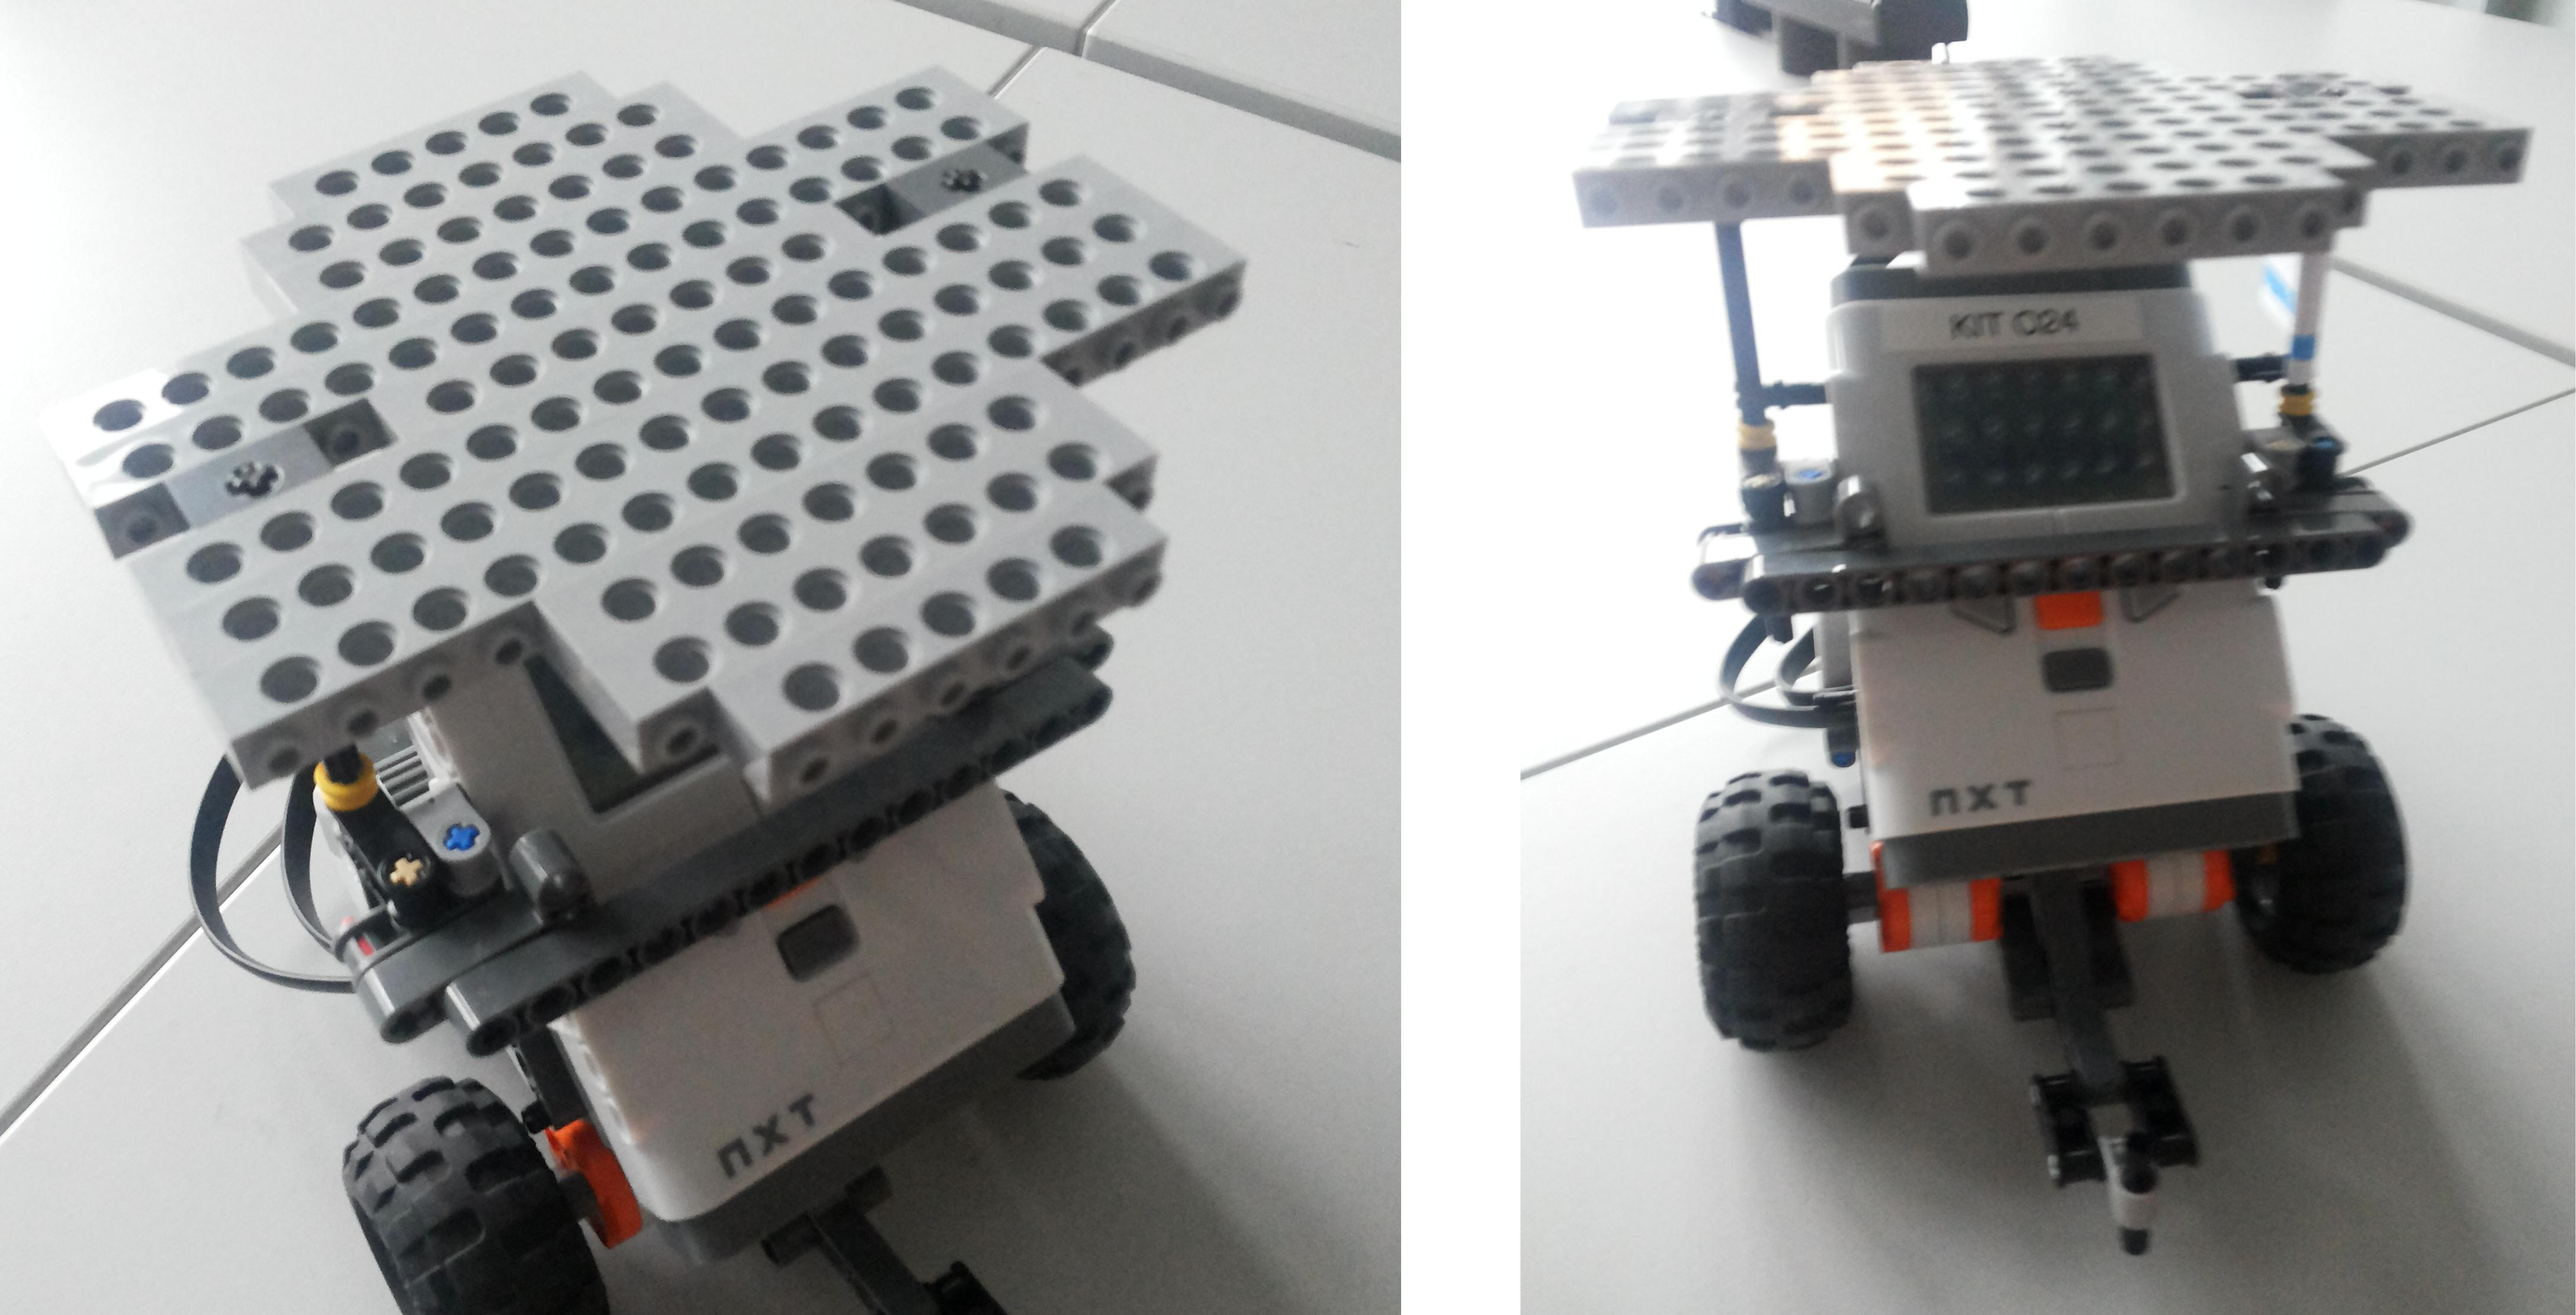
\includegraphics[width=0.5\textwidth]{markerHolder}
\end{figure}

One can see that the platform is wide enough for the marker, so it won't bend and the crossbar in the middle makes it not shaky. It was also placed in such a way so it will be as close as possible with the details we have to the robot's center of the mass so it won't outbalance it. Another important point is that the the markers must have a white frame around it, otherwise it will be detected inaccurately. First time we've tried to conduct an experiment using a wrong marker (Fig. \ref{fig:wrongMarker}) and the results were inacceptable -- in some positions cameras just have lost the robot. Therefore, we have changed the setup to leave some white field and used a smaller size, so it would be easier to mount it so it would be fatter, that one can see in Fig. \ref{fig:rightMarker}. In this case cameras didn't loose the robot in any position in the driving part of the room.

\begin{figure}[h]
  \centering
  \caption{A wrong marker mount.\label{fig:wrongMarker}}
  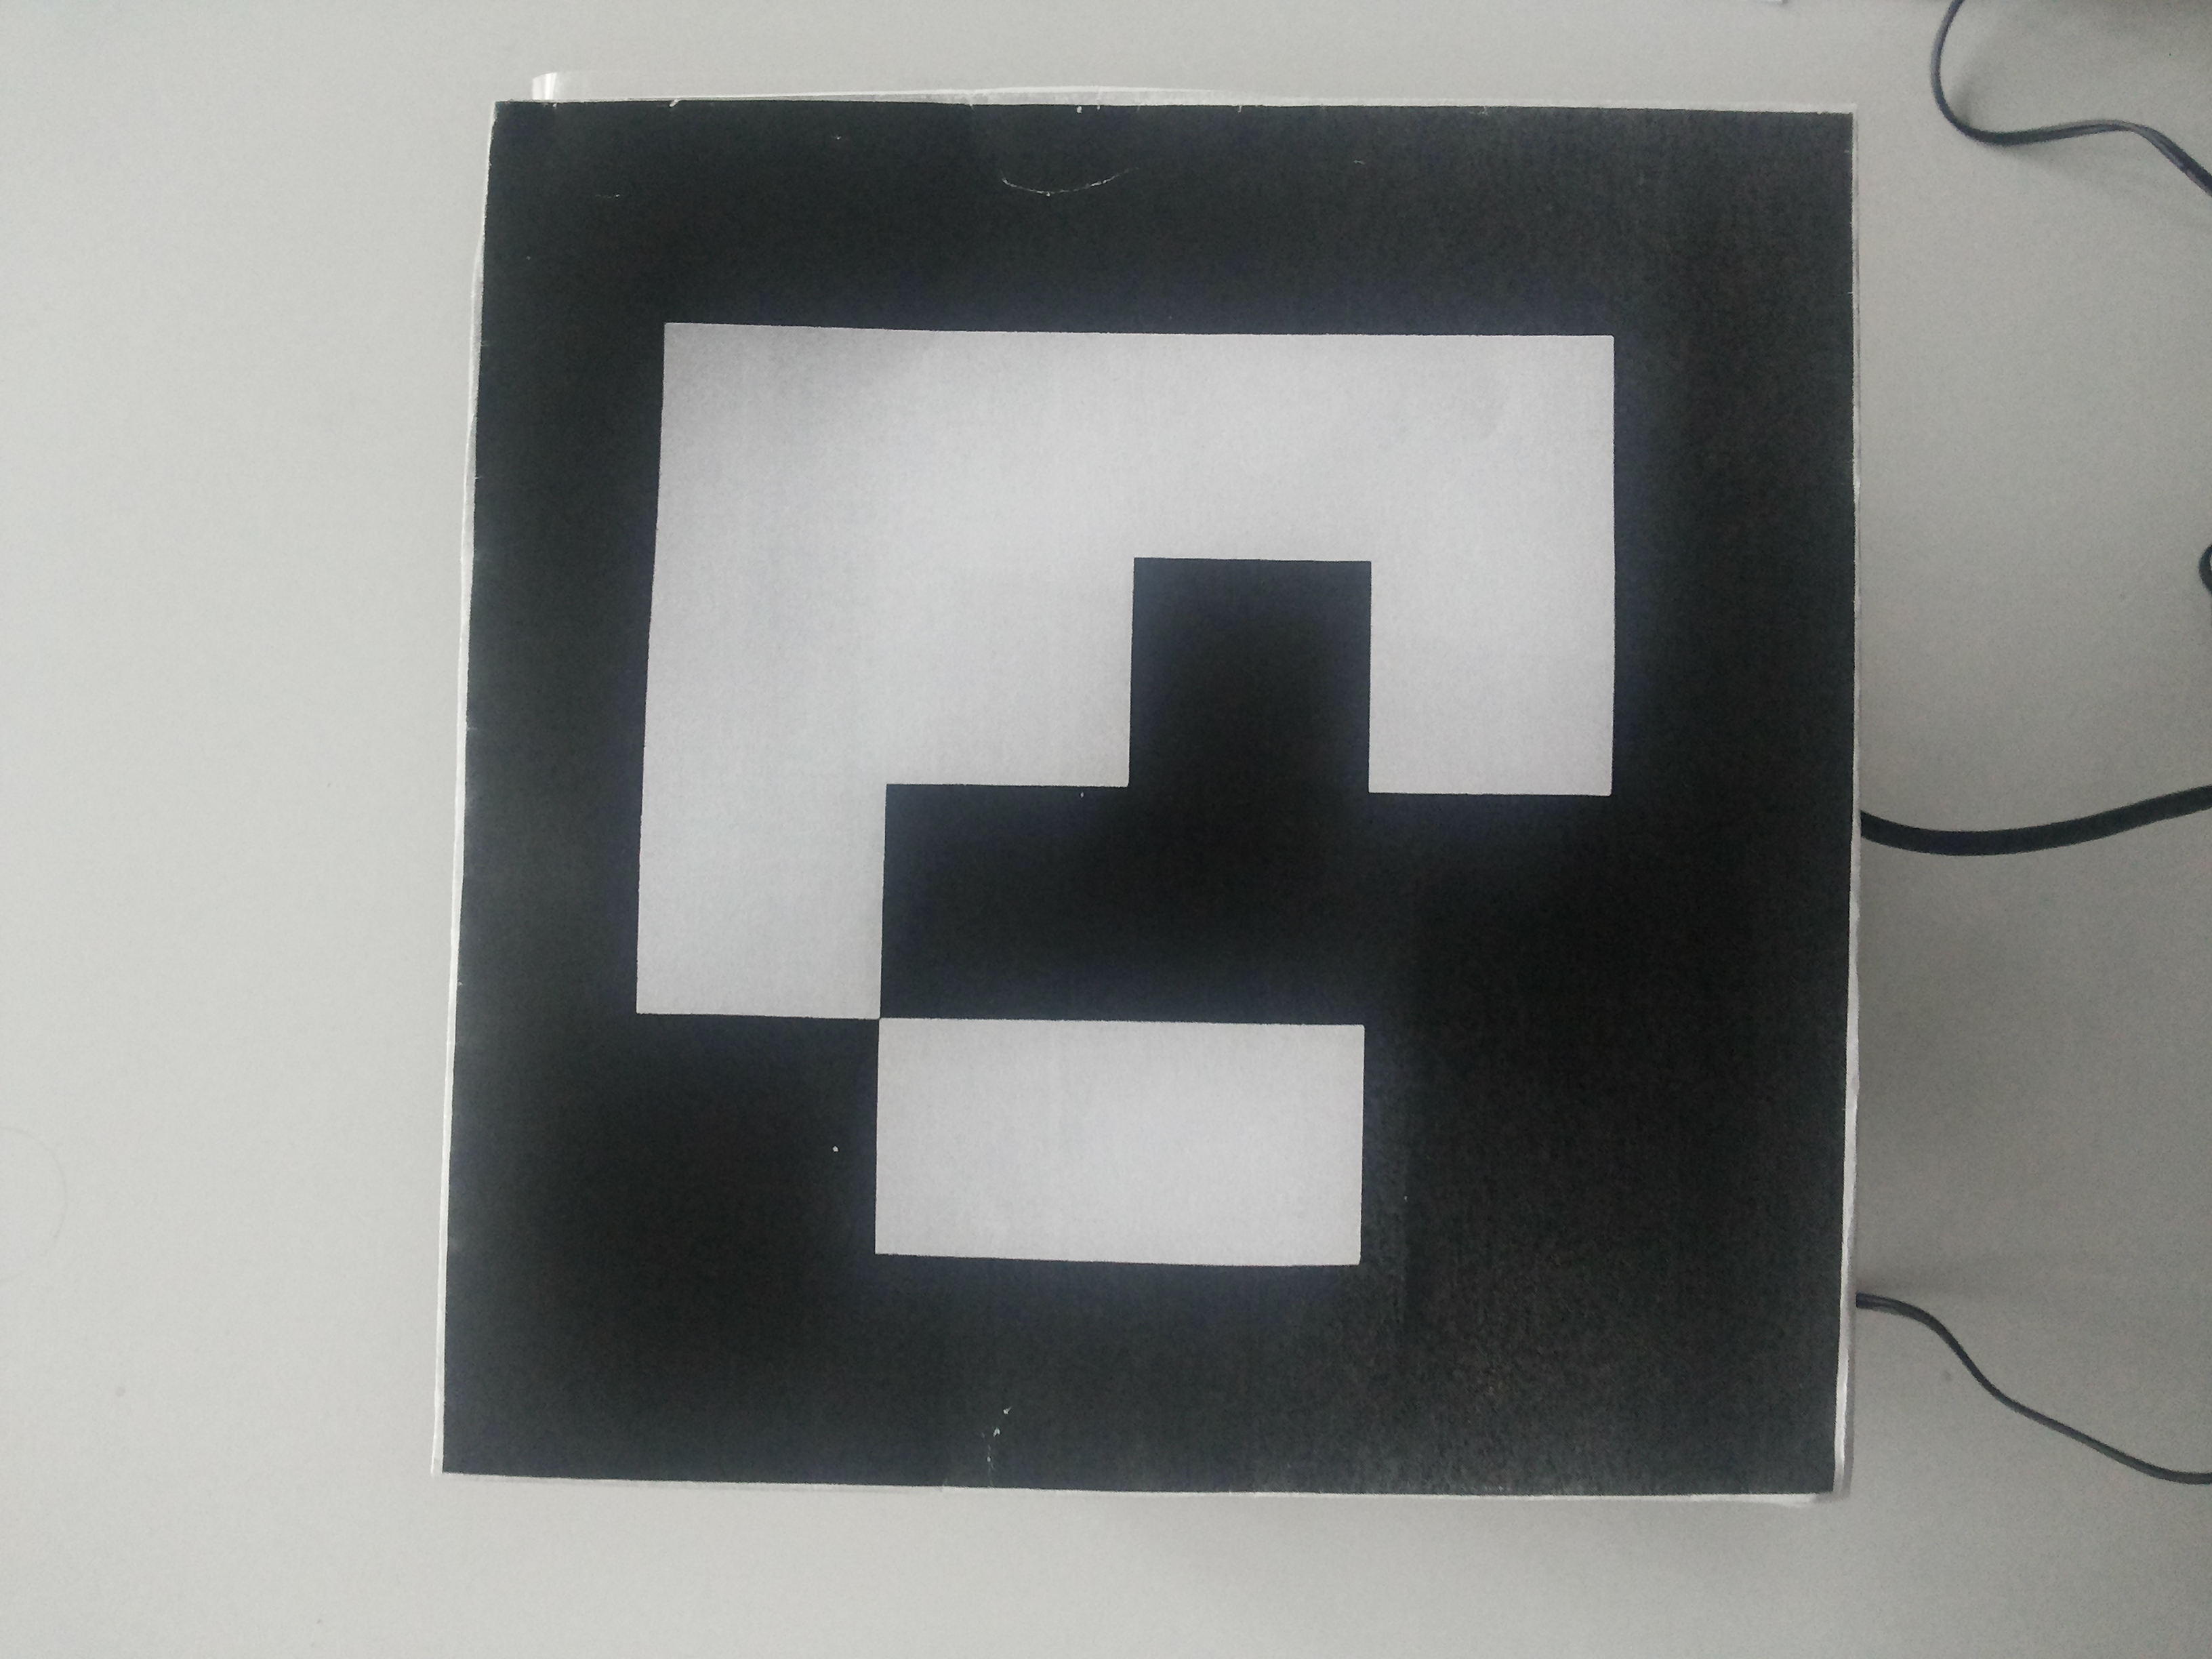
\includegraphics[width=0.3\textwidth]{wrongMarker}
\end{figure}

\begin{figure}[h]
  \centering
  \caption{A correct mount of the marker.\label{fig:rightMarker}}
  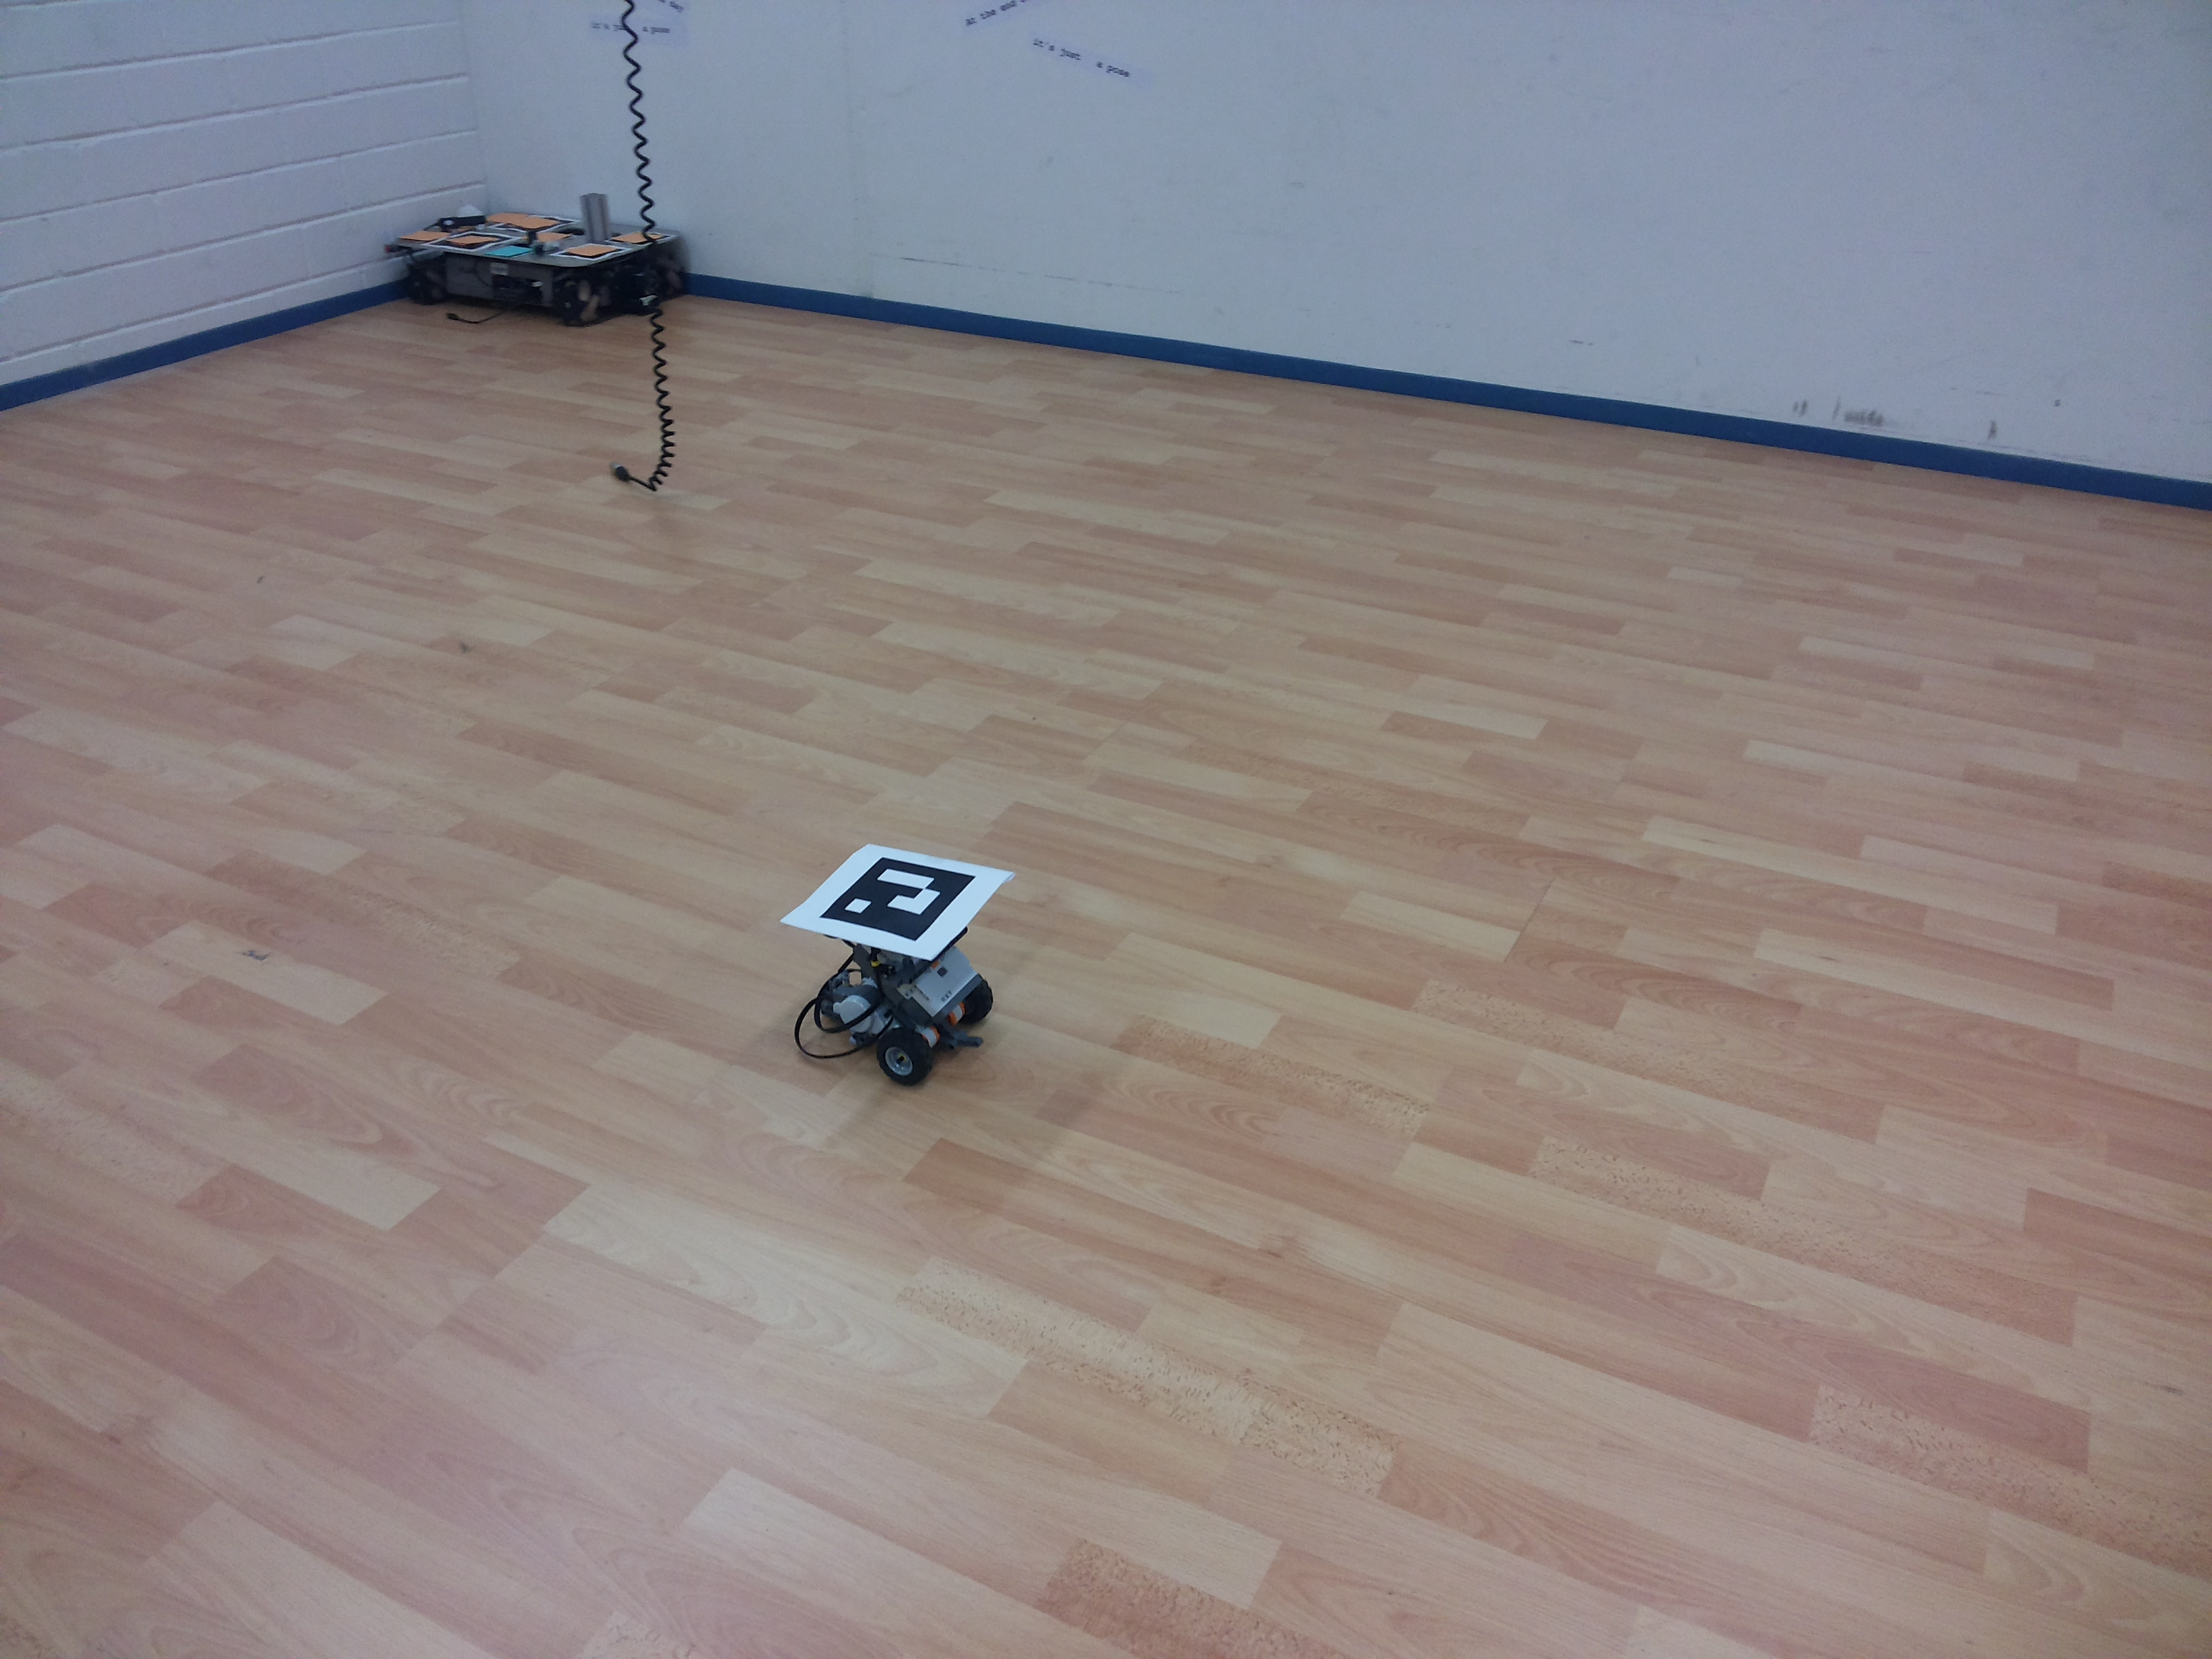
\includegraphics[width=0.5\textwidth]{rightMarker}
\end{figure}

To check if the system is working correctly, we've used a paper and a ruler in a way similar to the previous experiment on short distances, so the robot's motion error won't harm the results. The system was proven to be working correctly, however, the a number of simbols after comma in AICISS's measurement is much larger than we can possibly estimate by hands, so we cannot say anything about the exact precision of the system. \\

There are the following possible pitfalls:
\begin{itemize}
\item imperfections of the robot construction - since we are limited in details, it is hard to make a perfectly unshakable construction. We could not see it visually, but there could be a minor shaking that could affect the precision of the measurement
\item imperfection of robot's motors
\item problems related to a camera switching. To make it smoother we've used a video stitching tool (that can make a one video of three)
\item our robot is too small to mount multiple markers as it is done with youBot, so it has more problems with camera switching. If we would have tried to put more markers it would have either unbalance the system if it would have been on the top or harmed the motion if it would have been following the robot on some additional wheeled platform
\item imperfections of the cameras
\item the experiment took quite a lot of time, so the illumination changed
\item the camera calibration model perhaps not uses the skew (shear distortion), so if there is the one, it may cause the problems
\end{itemize}

\section{Program code}

It is sensible to make the measurements using the same parameters those we used in previous experiment. Construction of the robot wasn't changed much, so we'll be able to make a good comparison of the two ways of measurements. That is why we've left almost the same code, but without any light sensor activation and with the motion in loops. To distinguish different experimental tracks in the end of each loop step we've used a time delay of 5 seconds. So, if the position is not changing for this time, it is the end position of on track and start position of the second one. \\ 
For straight motion the robot moved eight times straight (approximately the length of the room), turned for  $180^{\circ}$ and went back. For arc motion robot moved clockwise and counterclockwise in two circles of different diameter (50 and 240 cm). We've used the following code:

 \begin{lstlisting}

package LegoNXT;

import lejos.nxt.LightSensor;
import lejos.nxt.Motor;
import lejos.nxt.SensorPort;
import lejos.robotics.navigation.DifferentialPilot;
import lejos.robotics.navigation.MoveController;
import lejos.util.Delay;
import lejos.nxt.Button;

public class goStraight {
	public static void main(String[] args) {
		double arcRad = 40;
		double angle = 90;
		double arcLen = Math.PI*2*arcRad*angle/360;
		double trackWidth = 12;
		DifferentialPilot dp = new DifferentialPilot(MoveController.WHEEL_SIZE_NXT1, trackWidth, Motor.B, Motor.C, true);
		Button.RIGHT.waitForPressAndRelease();
		for (int j = 0; j < 5; j++){
			for (int i = 0; i < 8; i++){
				dp.setTravelSpeed(10);
				dp.travel(-arcLen);   
				Delay.msDelay(5000);
			}
			dp.rotate(180);
		}
		Button.ESCAPE.waitForPressAndRelease();
	}
}



package LegoNXT;

import lejos.nxt.LightSensor;
import lejos.nxt.Motor;
import lejos.nxt.SensorPort;
import lejos.robotics.navigation.DifferentialPilot;
import lejos.robotics.navigation.MoveController;
import lejos.util.Delay;
import lejos.nxt.Button;

public class goRight {

	public static void main(String[] args) {
		double arcRad = 25;
		double angle = 90;
		double trackWidth = 12;
		DifferentialPilot dp = new DifferentialPilot(MoveController.WHEEL_SIZE_NXT1, trackWidth, Motor.B, Motor.C, true);
		Button.RIGHT.waitForPressAndRelease();
		for (int i = 0; i < 40; i++){
			dp.setTravelSpeed(10);
			dp.arc(arcRad, -angle);
			dp.stop();
			Delay.msDelay(5000);
		}
		Button.ESCAPE.waitForPressAndRelease();
	}
}


package LegoNXT;

import lejos.nxt.Motor;
import lejos.nxt.SensorPort;
import lejos.robotics.navigation.DifferentialPilot;
import lejos.robotics.navigation.MoveController;
import lejos.util.Delay;
import lejos.nxt.LightSensor;
import lejos.nxt.Button;

public class goLeft {

	public static void main(String[] args) {
		double arcRad = 25;
		double angle = 90;
		double trackWidth = 12;
		DifferentialPilot dp = new DifferentialPilot(MoveController.WHEEL_SIZE_NXT1, trackWidth, Motor.B, Motor.C, true);
		Button.RIGHT.waitForPressAndRelease();
		for (int i = 0; i < 40; i++){
			dp.setTravelSpeed(10);
			dp.arc(-arcRad, angle);
			dp.stop();
			Delay.msDelay(5000);
		}
		Button.ESCAPE.waitForPressAndRelease();
	}
}


package LegoNXT;

import lejos.nxt.Motor;
import lejos.nxt.SensorPort;
import lejos.robotics.navigation.DifferentialPilot;
import lejos.robotics.navigation.MoveController;
import lejos.util.Delay;
import lejos.nxt.LightSensor;
import lejos.nxt.Button;

public class goSlightlyRight {

	public static void main(String[] args) {
		double arcRad = 120;
		double angle = 30;
		double trackWidth = 12;
		DifferentialPilot dp = new DifferentialPilot(MoveController.WHEEL_SIZE_NXT1, trackWidth, Motor.B, Motor.C, true);
		Button.RIGHT.waitForPressAndRelease();
		for (int i = 0; i < 40; i++){
			dp.setTravelSpeed(10);
			dp.arc(arcRad, -angle);
			dp.stop();
			Delay.msDelay(5000);
		}
		Button.ESCAPE.waitForPressAndRelease();
	}
}


package LegoNXT;

import lejos.nxt.Button;
import lejos.nxt.LightSensor;
import lejos.nxt.Motor;
import lejos.nxt.SensorPort;
import lejos.robotics.navigation.DifferentialPilot;
import lejos.robotics.navigation.MoveController;
import lejos.util.Delay;

public class goSlightlyLeft {
	public static void main(String[] args) {
		double arcRad = 120;
		double angle = 30;
		double trackWidth = 12;
		DifferentialPilot dp = new DifferentialPilot(MoveController.WHEEL_SIZE_NXT1, trackWidth, Motor.B, Motor.C, true);
		Button.RIGHT.waitForPressAndRelease();
		
		for (int i = 0; i < 40; i++){
			dp.setTravelSpeed(10);
			dp.arc(-arcRad, angle);
			dp.stop();
			Delay.msDelay(5000);
		}
		Button.ESCAPE.waitForPressAndRelease();
	}
}



\end{lstlisting}

\section{Experimental results}

We've obtained the trajectories depicted in Fig. 

\begin{figure}[h]
  \centering
  \caption{Robot's trajectories: straight motion, left deep arc motion, right deep arc motion, left slight arc motion, right slight arc motion.\label{fig:trajectories}}
  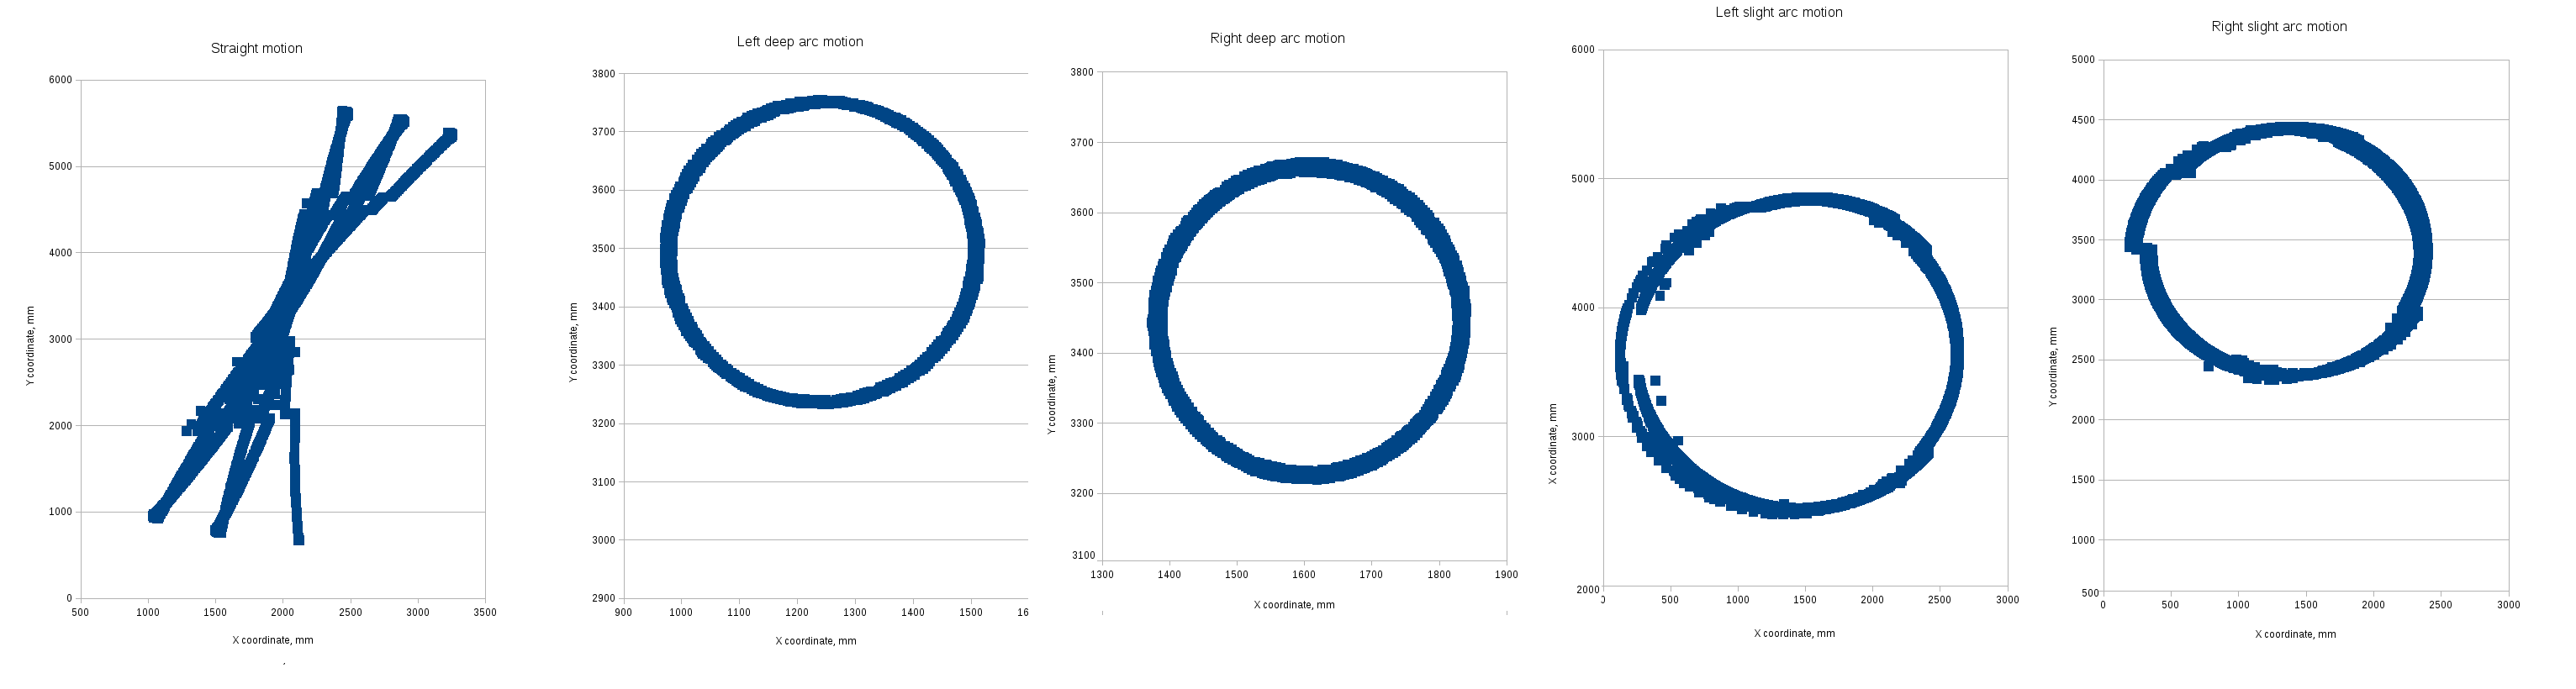
\includegraphics[width=1.0\textwidth]{trajectories}
\end{figure}

The results are in the attached excel files.

\section{Conclusion}

Small circles show quite a good result, because the whole path can be covered by one camera. In large circles and straight motion we see some breaking points those most likely appeared because of camera switch. We tried to avoid it by using camera stitcher tool, but apparently it could't fix it completely. Usage of multiple markers might help, but in the Lego robot case the markers should be either very small that can make their detection hard or mounted on the large platform that may harm the robot's balance. 


\end{document}
